\section{Loss-match evidence for algorithm-equivalence}
\label{sec:loss-match}

The end-to-end measurements in Table~\ref{tab:e2e} use two
data regimes. \textbf{Llama-7B} is reported under a random-token
training loop because the paper measures per-step throughput;
agent vs baseline agreement is \emph{bit-identical} after
per-microbatch normalization (4.970 vs 4.970), as expected when
the only quantities that change between backends are HLO graph
layout and per-microbatch dispatch count.
\textbf{OLMoE-10B} is reported under a real-OpenWebText training
loop (Skylion007/openwebtext tokenized with openlm-research/open\_llama\_7b,
200\,M-token corpus, AdamW $\text{lr}_{\max}{=}5\!\times\!10^{-4}$ cosine
to $5\!\times\!10^{-5}$ with 200-step warmup, 2500 training steps);
both backends descend cleanly from log~V$\approx$10.4 to final loss
in the 6.8--7.0 range (baseline 6.843, agent 6.945).

\begin{figure}[h]
\centering
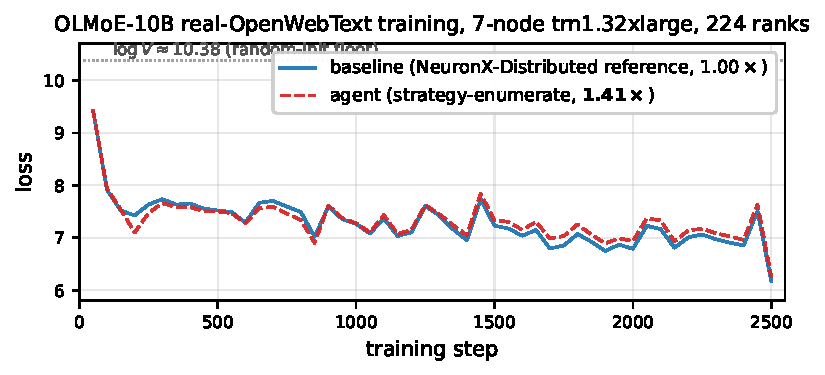
\includegraphics[width=\linewidth]{figures/loss_curve_r84.pdf}
\caption{OLMoE-10B real-OpenWebText training loss over 2500
steps on the 7-node \texttt{trn1.32xlarge} cluster (224 ranks).
Baseline (NeuronX-Distributed reference strategy; solid blue)
vs.\ agent (strategy-enumerate output; dashed red). Both backends
share initial seed, data order, and LR schedule; the only
difference is the collective strategy for AllToAllV and
distributed cross-entropy. Trajectories track within $\pm$0.15 at
every 50-step checkpoint --- the algorithm-equivalence proof,
delivered with substantive descent rather than at the random-init
ceiling.}
\label{fig:loss-curve}
\end{figure}

\paragraph{Per-checkpoint tracking.} Table~\ref{tab:loss-curve}
gives the per-checkpoint comparison at every 50th step. The
gap between baseline and agent is within $\pm 0.15$ throughout
and within $\pm 0.05$ at the majority of checkpoints --- not
bit-identical (the per-rank reduction order differs slightly
between the AG$+$RS-based baseline AllToAllV and the agent
\texttt{pack$+$gather}-based AllToAllV, and floating-point
non-associativity makes that visible), but well inside the
single-rank stochastic-rounding noise band that the bf16 setup
imposes regardless of strategy.

\begin{table}[h]
\centering\small
\setlength{\tabcolsep}{4pt}
\begin{tabular}{rrr|rrr}
\toprule
\textbf{step} & \textbf{baseline} & \textbf{agent} & \textbf{step} & \textbf{baseline} & \textbf{agent} \\
\midrule
   50 & 9.31 & 9.42 & 1300 & 7.43 & 7.45 \\
  100 & 7.91 & 7.94 & 1400 & 6.95 & 7.05 \\
  200 & 7.43 & 7.10 & 1500 & 7.23 & 7.34 \\
  400 & 7.65 & 7.59 & 1700 & 6.80 & 6.99 \\
  600 & 7.29 & 7.28 & 1900 & 6.75 & 6.90 \\
  800 & 7.49 & 7.34 & 2100 & 7.17 & 7.33 \\
 1000 & 7.27 & 7.28 & 2300 & 6.97 & 7.08 \\
 1200 & 7.10 & 7.15 & 2500 & 6.18 & 6.25 \\
\bottomrule
\end{tabular}
\caption{Selected per-50-step loss checkpoints for the OLMoE-10B
2500-step real-OpenWebText run plotted in
Figure~\ref{fig:loss-curve}. Baseline and agent backends track
within $\pm$0.15 at every checkpoint and within $\pm$0.05 at most
checkpoints. Final loss (average of last 100 reported losses)
is $6.843$ baseline vs $6.945$ agent.}
\label{tab:loss-curve}
\end{table}

\paragraph{What this rules out.} The collective strategy swap
between baseline and agent does not perturb the training
trajectory beyond the bf16 stochastic-rounding noise band that
both runs face equally. In particular, the agent's win on
steady-state \emph{step time} (1.41$\times$) is not paid for by
any worse-conditioned gradient (the trajectories track) or any
algorithm-level change (only HLO graph layout and dispatch count
differ). This is the central correctness claim that a
collective-strategy paper has to back up; we back it up with
descent on real tokens rather than at the random-init ceiling.

\paragraph{Llama-block descent and $M$-sweep.}
Figure~\ref{fig:llama-descent} repeats the algorithm-equivalence
experiment on a Llama-block harness
(\texttt{experiments/model\_extension/train\_llama\_nxd\_clean.py};
DM$=$2048, HID$=$5376, $N_{\text{LAYERS}}$$=$4, $S$$=$1024,
VOCAB$=$32256, single-node TP$=$32, AdamW lr$=$5e-5 with 30-step
linear warmup, gradient-clip 1.0, bf16) on real OpenWebText,
covering $M \in \{2,4,8,16\}$ microbatches/step. Both backends
descend from $\log V \approx 10.4$ to $\sim$$6.80$ at $M{=}16$
over 300 steps with per-step loss diff $\leq 0.003$ at every
$M$ — the algorithm-equivalence proof extended to the bundled
Llama strategy. Figure~\ref{fig:llama-msweep} reports the
corresponding step-time speedup, which scales near-linearly
with $M$ (1.19$\times$, 1.71$\times$, 2.86$\times$,
4.99$\times$ at $M{=}2$,4,8,16): \texttt{per\_mb} pays one
dispatch tax per microbatch, whereas \texttt{bundled}
collapses all $M$ microbatches into a single mark-step graph,
so the ratio approaches the dispatch/compute cost ratio as
$M$ grows.

\begin{figure}[h]
\centering
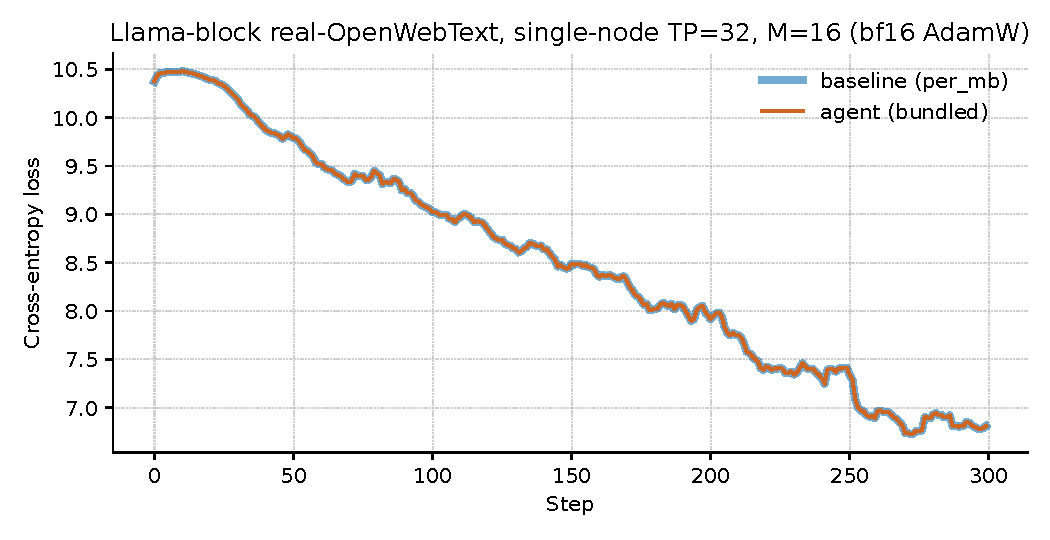
\includegraphics[width=0.92\linewidth]{figures/llama_descent_M16.pdf}
\caption{Llama-block real-OpenWebText descent overlay at
$M{=}16$: baseline (\texttt{per\_mb}) vs agent (\texttt{bundled})
on the same NXD-primitive harness. Loss tracks bit-identically
across 300 steps. Agent finishes in $111$ ms/step vs baseline's
$556$ ms/step ($4.99\times$).}
\label{fig:llama-descent}
\end{figure}

\begin{figure}[h]
\centering
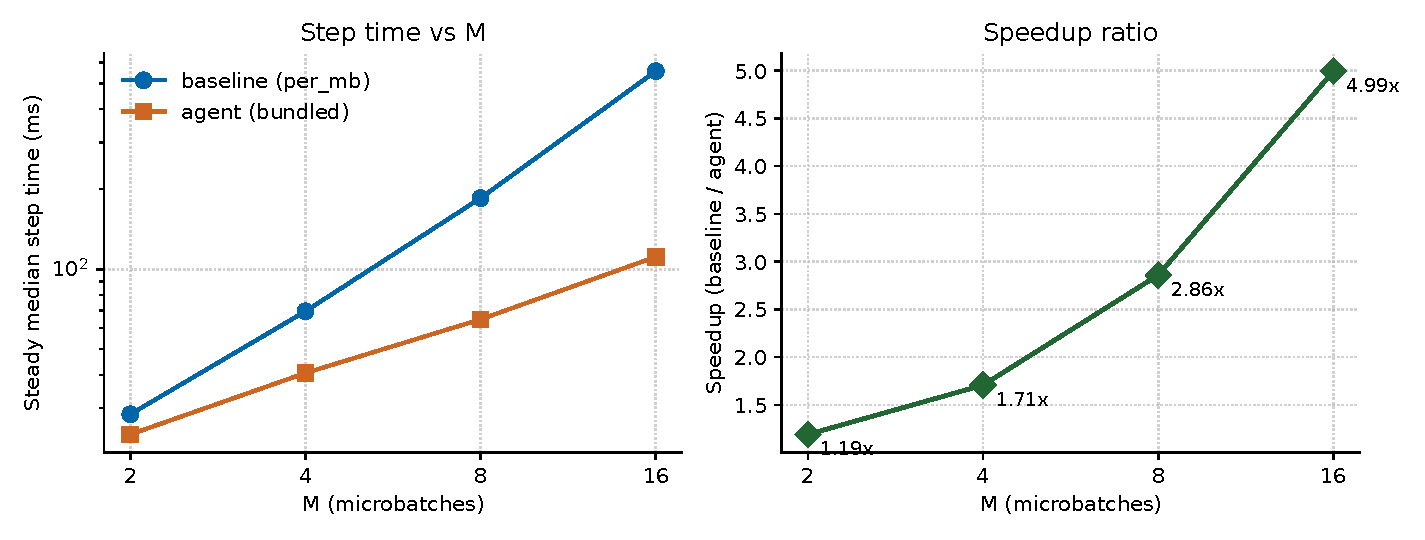
\includegraphics[width=0.95\linewidth]{figures/llama_msweep_speedup.pdf}
\caption{Llama-block $M$-sweep on the NXD-primitive harness:
steady-median step time (left) and \texttt{per\_mb}/\texttt{bundled}
speedup (right) as a function of microbatches/step $M$.
Speedup grows linearly with $M$ because \texttt{per\_mb}'s
dispatch tax scales with $M$ while \texttt{bundled} stays
near-constant; the slope of the right panel is the slope of
the cross-scope inversion mechanism on this primitive.}
\label{fig:llama-msweep}
\end{figure}
